\documentclass[11pt,a4paper]{report}
\usepackage[textwidth=37em,vmargin=30mm]{geometry}
\usepackage{calc,xunicode,amsmath,amssymb,paralist,enumitem,tabu,booktabs,datetime2,xeCJK,xeCJKfntef,listings}
\usepackage{tocloft,fancyhdr,tcolorbox,xcolor,graphicx,eso-pic,xltxtra,xelatexemoji}

\newcommand{\envyear}[0]{2025}
\newcommand{\envdatestr}[0]{2025-06-01}
\newcommand{\envfinaldir}[0]{webdb/2025/20250601/final}

\usepackage[hidelinks]{hyperref}
\hypersetup{
    colorlinks=false,
    pdfpagemode=FullScreen,
    pdftitle={Web Digest - \envdatestr}
}

\setlength{\cftbeforechapskip}{10pt}
\renewcommand{\cftchapfont}{\rmfamily\bfseries\large\raggedright}
\setlength{\cftbeforesecskip}{2pt}
\renewcommand{\cftsecfont}{\sffamily\small\raggedright}

\setdefaultleftmargin{2em}{2em}{1em}{1em}{1em}{1em}

\usepackage{xeCJK,xeCJKfntef}
\xeCJKsetup{PunctStyle=plain,RubberPunctSkip=false,CJKglue=\strut\hskip 0pt plus 0.1em minus 0.05em,CJKecglue=\strut\hskip 0.22em plus 0.2em}
\XeTeXlinebreaklocale "zh"
\XeTeXlinebreakskip = 0pt


\setmainfont{Brygada 1918}
\setromanfont{Brygada 1918}
\setsansfont{IBM Plex Sans}
\setmonofont{JetBrains Mono NL}
\setCJKmainfont{Noto Serif CJK SC}
\setCJKromanfont{Noto Serif CJK SC}
\setCJKsansfont{Noto Sans CJK SC}
\setCJKmonofont{Noto Sans CJK SC}

\setlength{\parindent}{0pt}
\setlength{\parskip}{8pt}
\linespread{1.15}

\lstset{
	basicstyle=\ttfamily\footnotesize,
	numbersep=5pt,
	backgroundcolor=\color{black!5},
	showspaces=false,
	showstringspaces=false,
	showtabs=false,
	tabsize=2,
	captionpos=b,
	breaklines=true,
	breakatwhitespace=true,
	breakautoindent=true,
	linewidth=\textwidth
}






\newcommand{\coverpic}[2]{
    % argv: itemurl, authorname
    Cover photo by #2~~(\href{#1}{#1})
}
\newcommand{\makeheader}[0]{
    \begin{titlepage}
        % \newgeometry{hmargin=15mm,tmargin=21mm,bmargin=12mm}
        \begin{center}
            
            \rmfamily\scshape
            \fontspec{BaskervilleF}
            \fontspec{Old Standard}
            \fontsize{59pt}{70pt}\selectfont
            WEB\hfill DIGEST
            
            \vfill
            % \vskip 30pt
            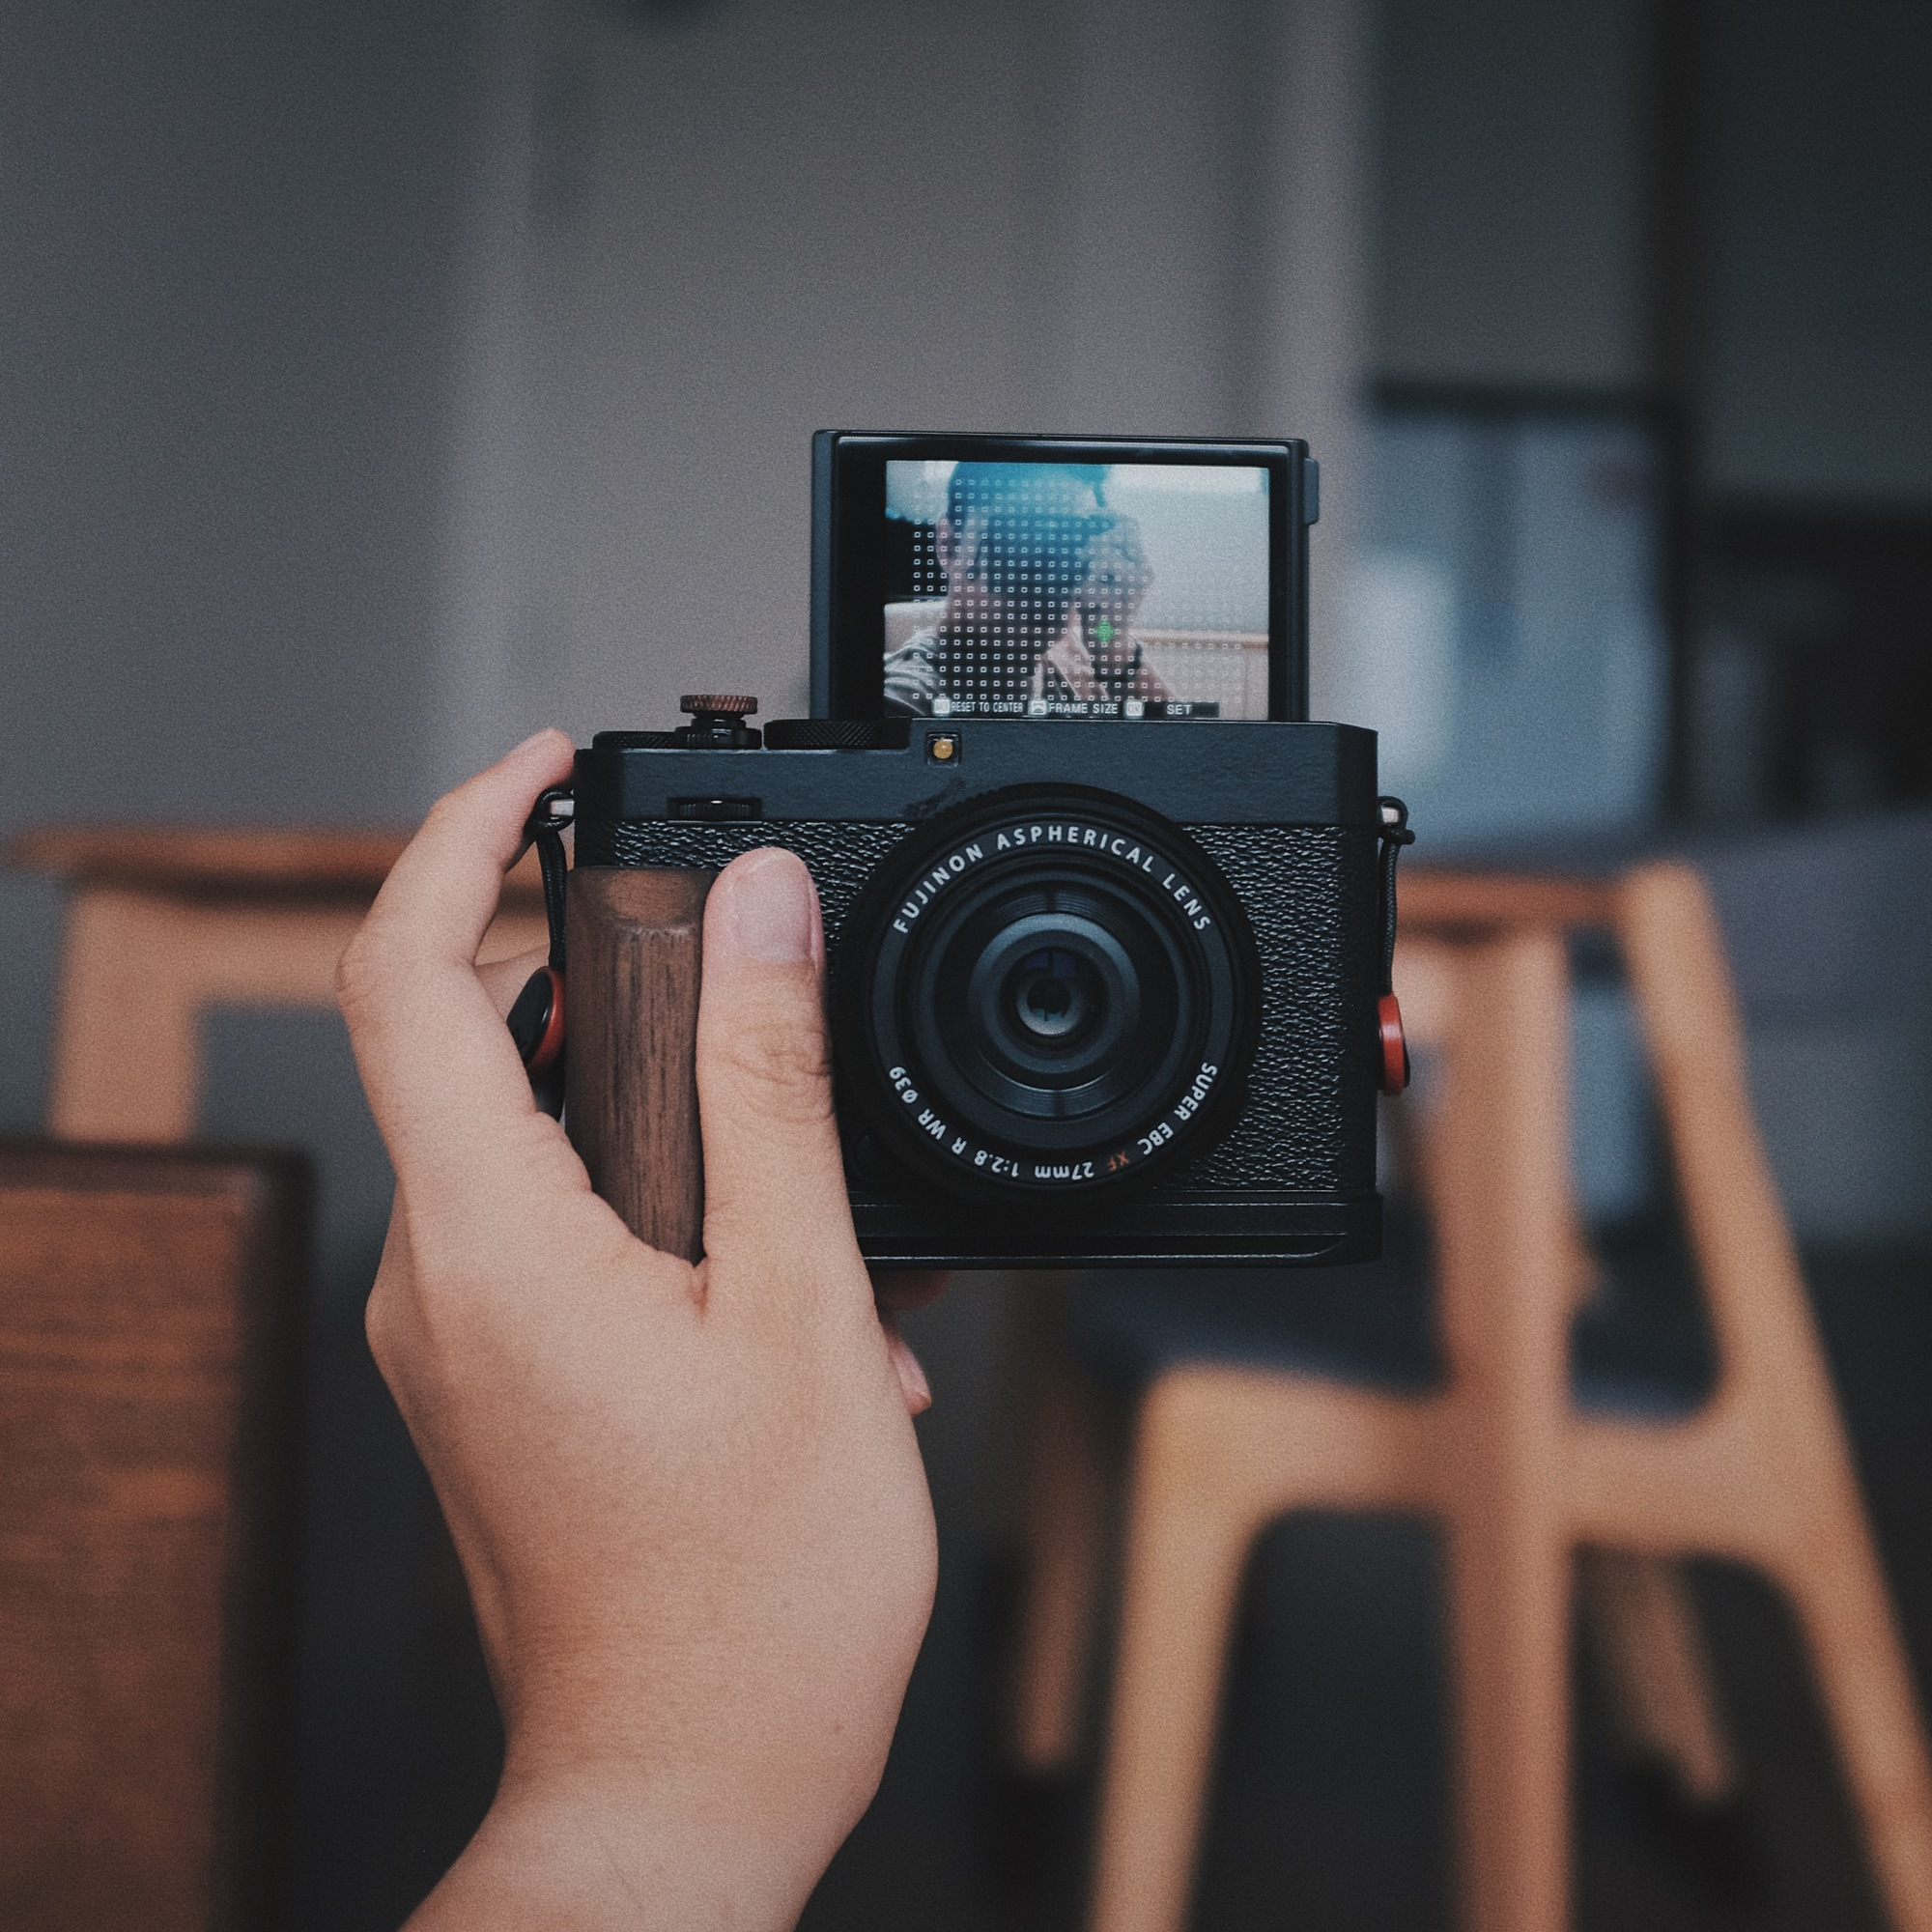
\includegraphics[width=\linewidth]{\envfinaldir/coverpic-prod.jpg}\par
            % \vskip 30pt
            \vfill

            \normalsize\rmfamily\scshape
            \copyright{} The Web Digest Project \hfill\large \envdatestr
        \end{center}
    \end{titlepage}
    % \restoregeometry
}
\newcommand{\simplehref}[1]{%
    \textcolor{blue!80!green}{\href{#1}{#1}}%
}
\renewcommand{\contentsname}{\center\Huge\sffamily\bfseries Contents\par\vskip 20pt}
\newcounter{ipartcounter}
\setcounter{ipartcounter}{0}
\newcommand{\ipart}[1]{
    % \vskip 20pt
    \clearpage
    \stepcounter{ipartcounter}
    \phantomsection
    \addcontentsline{toc}{chapter}{#1}
    % \begin{center}
    %     \Huge
    %     \sffamily\bfseries
    %     #1
    % \end{center}
    % \vskip 20pt plus 7pt
}
\newcounter{ichaptercounter}
\setcounter{ichaptercounter}{0}
\newcommand{\ichapter}[1]{
    % \vskip 20pt
    \clearpage
    \stepcounter{ichaptercounter}
    \phantomsection
    \addcontentsline{toc}{section}{\numberline{\arabic{ichaptercounter}}#1}
    \begin{center}
        \Huge
        \sffamily\bfseries
        #1
    \end{center}
    \vskip 20pt plus 7pt
}
\newcommand{\entrytitlefont}[1]{\subsection*{\raggedright\Large\sffamily\bfseries#1}}
\newcommand{\entryitemGeneric}[2]{
    % argv: title, url
    \parbox{\linewidth}{
        \entrytitlefont{#1}\par\vskip 5pt
        \footnotesize\ttfamily\mdseries
        \simplehref{#2}
    }\vskip 11pt plus 11pt minus 1pt
}
\newcommand{\entryitemGithub}[3]{
    % argv: title, url, desc
    \parbox{\linewidth}{
        \entrytitlefont{#1}\par\vskip 5pt
        \footnotesize\ttfamily\mdseries
        \simplehref{#2}\par\vskip 5pt
        \small\rmfamily\mdseries#3
    }\vskip 11pt plus 11pt minus 1pt
}
\newcommand{\entryitemAp}[3]{
    % argv: title, url, desc
    \parbox{\linewidth}{
        \entrytitlefont{#1}\par\vskip 5pt
        \footnotesize\ttfamily\mdseries
        \simplehref{#2}\par\vskip 5pt
        \small\rmfamily\mdseries#3
    }\vskip 11pt plus 11pt minus 1pt
}
\newcommand{\entryitemHackernews}[3]{
    % argv: title, hnurl, rawurl
    % \parbox{\linewidth}{
    %     \entrytitlefont{#1}\par\vskip 5pt
    %     \footnotesize\ttfamily\mdseries
    %     \simplehref{#3}\par
    %     \textcolor{black!50}{\href{#2}{#2}}
    % }\vskip 11pt plus 11pt minus 1pt
    \begin{minipage}{\linewidth}
            \entrytitlefont{#1}\par\vskip 5pt
            \footnotesize\ttfamily\mdseries
            \simplehref{#3}\par
            \textcolor{black!50}{\href{#2}{#2}}
    \end{minipage}\par\vskip 11pt plus 11pt minus 1pt
}







\begin{document}

\makeheader

\tableofcontents\clearpage




\ipart{Developers}
\ichapter{Hacker News}
\entryitemTwoLinks{A Lean companion to Analysis I}{https://news.ycombinator.com/item?id=44145517}{https://terrytao.wordpress.com/2025/05/31/a-lean-companion-to-analysis-i/}

\entryitemTwoLinks{Precision Clock Mk IV}{https://news.ycombinator.com/item?id=44144750}{https://mitxela.com/projects/precision\_clock\_mk\_iv}

\entryitemTwoLinks{Ask HN: Anyone making a living from a paid API?}{https://news.ycombinator.com/item?id=44144473}{https://news.ycombinator.com/item?id=44144473}

\entryitemTwoLinks{Doge cuts to USAid blamed for 300k deaths – most of them children}{https://news.ycombinator.com/item?id=44142790}{https://www.thetimes.com/us/american-politics/article/usaid-doge-deaths-children-cuts-7nb83dfkp}

\entryitemTwoLinks{Using lots of little tools to aggressively reject the bots}{https://news.ycombinator.com/item?id=44142761}{https://lambdacreate.com/posts/68}

\entryitemTwoLinks{Beware of Fast-Math}{https://news.ycombinator.com/item?id=44142472}{https://simonbyrne.github.io/notes/fastmath/}

\entryitemTwoLinks{Gradients Are the New Intervals}{https://news.ycombinator.com/item?id=44142266}{https://www.mattkeeter.com/blog/2025-05-14-gradients/}

\entryitemTwoLinks{AI Responses May Include Mistakes}{https://news.ycombinator.com/item?id=44142113}{https://www.os2museum.com/wp/ai-responses-may-include-mistakes/}

\entryitemTwoLinks{Simpler Backoff}{https://news.ycombinator.com/item?id=44141887}{https://commaok.xyz/post/simple-backoff/}

\entryitemTwoLinks{Every 5x5 Nonogram}{https://news.ycombinator.com/item?id=44140918}{https://pixelogic.app/every-5x5-nonogram}

\entryitemTwoLinks{Valkey Turns One: Community fork of Redis}{https://news.ycombinator.com/item?id=44140379}{https://www.gomomento.com/blog/valkey-turns-one-how-the-community-fork-left-redis-in-the-dust/}

\entryitemTwoLinks{Silicon Valley finally has a big electronics retailer again: Micro Center opens}{https://news.ycombinator.com/item?id=44140378}{https://www.microcenter.com/site/mc-news/article/micro-center-santa-clara-photos.aspx}

\entryitemTwoLinks{C++ to Rust Phrasebook}{https://news.ycombinator.com/item?id=44140349}{https://cel.cs.brown.edu/crp/}

\entryitemTwoLinks{Photos taken inside musical instruments}{https://news.ycombinator.com/item?id=44139626}{https://www.dpreview.com/photography/5400934096/probe-lenses-and-focus-stacking-the-secrets-to-incredible-photos-taken-inside-instruments}

\entryitemTwoLinks{Jerry Lewis's ``The Day the Clown Cried'' discovered in Sweden after 53 years}{https://news.ycombinator.com/item?id=44139592}{https://www.thenationalnews.com/arts-culture/film-tv/2025/05/29/jerry-lewis-day-the-clown-cried-discovered/}

\entryitemTwoLinks{Surprisingly fast AI-generated kernels we didn't mean to publish yet}{https://news.ycombinator.com/item?id=44139454}{https://crfm.stanford.edu/2025/05/28/fast-kernels.html}

\entryitemTwoLinks{Mary Meeker's first Trends report since 2019, focused on AI}{https://news.ycombinator.com/item?id=44139403}{https://www.bondcap.com/reports/tai}

\entryitemTwoLinks{Cap: Lightweight, modern open-source CAPTCHA alternative using proof-of-work}{https://news.ycombinator.com/item?id=44137867}{https://capjs.js.org/}

\entryitemTwoLinks{Beating Google's kernelCTF PoW using AVX512}{https://news.ycombinator.com/item?id=44137715}{https://anemato.de/blog/kctf-vdf}

\entryitemTwoLinks{Toxic Origins, Toxic Decisions: Biases in CEO Selection}{https://news.ycombinator.com/item?id=44137542}{https://papers.ssrn.com/sol3/papers.cfm?abstract\_id=5270031}\ichapter{Phoronix}
\entryitemGeneric{\hskip 0pt{}Linux 6.16 Now Enforces A Minimum Compiler Version Of GCC 8}{https://www.phoronix.com/news/Linux-6.16-Requires-GCC-8-Min}

\entryitemGeneric{\hskip 0pt{}Linux 6.16 Enabling Support For 11 More SoCs, Sophgo SG2044 \& More Snapdragon X Laptops}{https://www.phoronix.com/news/Linux-6.16-SoCs}

\entryitemGeneric{\hskip 0pt{}AMD ROCm 7.0 To Align HIP C++ "Even More Closely With CUDA"}{https://www.phoronix.com/news/AMD-ROCm-7.0-HIP-Plans}

\entryitemGeneric{\hskip 0pt{}Linux's Trusted Security Manager Sees First Updates In Over A Year}{https://www.phoronix.com/news/Linux-6.16-TSM}

\entryitemGeneric{\hskip 0pt{}CachyOS Improves NVIDIA Driver Loading, Better Handheld Device Support}{https://www.phoronix.com/news/CachyOS-May-2025-Release}

\entryitemGeneric{\hskip 0pt{}A Few New Media Drivers Land In Linux 6.16}{https://www.phoronix.com/news/Linux-6.16-Media-Drivers}

\entryitemGeneric{\hskip 0pt{}KDE Plasma 6.5 Will Help Reduce RAM Use By Keeping Less Wallpaper Copies Around}{https://www.phoronix.com/news/Plasma-6.5-Less-Wallpaper-RAM}

\entryitemGeneric{\hskip 0pt{}Intel PTC, Intel EAS \& AMD Requested CPU Min Freq Features Merged For Linux 6.16}{https://www.phoronix.com/news/Linux-6.16-Power-Management}

\entryitemGeneric{\hskip 0pt{}Intel Prepping Linux Driver For Future Data Center GPUs Based On Battlemage}{https://www.phoronix.com/news/Intel-Future-DC-GPU-Linux-BMG}\ichapter{Dribbble}
\entryitemGeneric{\hskip 0pt{}Cre8tera // Website}{https://dribbble.com/shots/26091009-Cre8tera-Website}

\entryitemGeneric{\hskip 0pt{}Singular Logo Concept (Unused)}{https://dribbble.com/shots/26091755-Singular-Logo-Concept-Unused}

\entryitemGeneric{\hskip 0pt{}Mnp Technologies - Logo Design}{https://dribbble.com/shots/26092034-Mnp-Technologies-Logo-Design}

\entryitemGeneric{\hskip 0pt{}zeero logo design}{https://dribbble.com/shots/26087342-zeero-logo-design}

\entryitemGeneric{\hskip 0pt{}Eagle}{https://dribbble.com/shots/26085536-Eagle}

\entryitemGeneric{\hskip 0pt{}Shori Brand}{https://dribbble.com/shots/26088139-Shori-Brand}

\entryitemGeneric{\hskip 0pt{}Create email inbox composition}{https://dribbble.com/shots/26083118-Create-email-inbox-composition}

\entryitemGeneric{\hskip 0pt{}Roaring Bear}{https://dribbble.com/shots/26087788-Roaring-Bear}

\entryitemGeneric{\hskip 0pt{}Hand-drawn illustration pack}{https://dribbble.com/shots/26084735-Hand-drawn-illustration-pack}

\entryitemGeneric{\hskip 0pt{}B2B Dashboard \& Web App UI UX Design for Carbon Solutions}{https://dribbble.com/shots/26076624-B2B-Dashboard-Web-App-UI-UX-Design-for-Carbon-Solutions}

\entryitemGeneric{\hskip 0pt{}Patriot Logo Design (Unused for Sale)}{https://dribbble.com/shots/26081047-Patriot-Logo-Design-Unused-for-Sale}

\entryitemGeneric{\hskip 0pt{}Apple}{https://dribbble.com/shots/26084067-Apple}

\entryitemGeneric{\hskip 0pt{}Illustration}{https://dribbble.com/shots/26083223-Illustration}

\entryitemGeneric{\hskip 0pt{}Heliopoint}{https://dribbble.com/shots/26081987-Heliopoint}

\entryitemGeneric{\hskip 0pt{}Heyo Turns 2!}{https://dribbble.com/shots/26078572-Heyo-Turns-2}

\entryitemGeneric{\hskip 0pt{}Roaring Bear}{https://dribbble.com/shots/26077332-Roaring-Bear}

\entryitemGeneric{\hskip 0pt{}Smart Home App}{https://dribbble.com/shots/26076565-Smart-Home-App}

\entryitemGeneric{\hskip 0pt{}Fox Brand Mascot}{https://dribbble.com/shots/26077954-Fox-Brand-Mascot}

\entryitemGeneric{\hskip 0pt{}Game Studio Logo}{https://dribbble.com/shots/26076821-Game-Studio-Logo}

\entryitemGeneric{\hskip 0pt{}HYDRO - Logo Design}{https://dribbble.com/shots/26073470-HYDRO-Logo-Design}

\entryitemGeneric{\hskip 0pt{}Credit payment card bank app animation}{https://dribbble.com/shots/26063214-Credit-payment-card-bank-app-animation}

\entryitemGeneric{\hskip 0pt{}S}{https://dribbble.com/shots/26071612-S}

\entryitemGeneric{\hskip 0pt{}Dedicated to Dumplings}{https://dribbble.com/shots/26073310-Dedicated-to-Dumplings}

\entryitemGeneric{\hskip 0pt{}Project Management Dashboard}{https://dribbble.com/shots/26070177-Project-Management-Dashboard}


\ipart{Developers~~~~(zh-Hans)}
\ichapter{Solidot}
\entryitemGeneric{\hskip 0pt{}印度严重的空气污染无意中起到了降温作用}{https://www.solidot.org/story?sid=81437}

\entryitemGeneric{\hskip 0pt{}白宫的健康报告被发现部分内容是大模型生成的}{https://www.solidot.org/story?sid=81436}

\entryitemGeneric{\hskip 0pt{}美国禁止向中国出售半导体设计软件}{https://www.solidot.org/story?sid=81435}

\entryitemGeneric{\hskip 0pt{}Stack Overflow 将测试付费给专家回答问题}{https://www.solidot.org/story?sid=81434}

\entryitemGeneric{\hskip 0pt{}SEC 撤销对币安的诉讼}{https://www.solidot.org/story?sid=81433}

\entryitemGeneric{\hskip 0pt{}全球气温到 2029 年可能首次升温超 2℃}{https://www.solidot.org/story?sid=81432}

\entryitemGeneric{\hskip 0pt{}研究人员认为大模型既不会思考也不会推理}{https://www.solidot.org/story?sid=81431}

\entryitemGeneric{\hskip 0pt{}惠普将停止在中国制造销往北美的产品}{https://www.solidot.org/story?sid=81430}

\entryitemGeneric{\hskip 0pt{}通过饮料摄入糖比食用糖对健康危害更大}{https://www.solidot.org/story?sid=81429}

\entryitemGeneric{\hskip 0pt{}天问二号将执行小行星取样任务}{https://www.solidot.org/story?sid=81428}

\entryitemGeneric{\hskip 0pt{}组合使用两种抗衰老药物延长小鼠寿命三成}{https://www.solidot.org/story?sid=81427}

\entryitemGeneric{\hskip 0pt{}微软向第三方应用开放 Windows Update }{https://www.solidot.org/story?sid=81426}

\entryitemGeneric{\hskip 0pt{}日本邮政推出数字地址}{https://www.solidot.org/story?sid=81425}

\entryitemGeneric{\hskip 0pt{}甲骨文通过 GitHub 发布 VirtualBox 源代码}{https://www.solidot.org/story?sid=81424}

\entryitemGeneric{\hskip 0pt{}数千华硕路由器感染了难以清除的后门}{https://www.solidot.org/story?sid=81423}

\entryitemGeneric{\hskip 0pt{}苹果操作系统将用年份标识版本号}{https://www.solidot.org/story?sid=81422}

\entryitemGeneric{\hskip 0pt{}为什么我们遵守规则?}{https://www.solidot.org/story?sid=81421}

\entryitemGeneric{\hskip 0pt{}美国将撤销中国留学生签证}{https://www.solidot.org/story?sid=81420}

\entryitemGeneric{\hskip 0pt{}xAI 支付 3 亿美元让 Telegram 集成 Grok}{https://www.solidot.org/story?sid=81419}

\entryitemGeneric{\hskip 0pt{}我们如何失去互联网?}{https://www.solidot.org/story?sid=81418}\ichapter{V2EX}
\entryitemGeneric{\hskip 0pt{}[Notes] 周经帖的末日?笔记软件已经进入决赛圈}{https://www.v2ex.com/t/1135671}

\entryitemGeneric{\hskip 0pt{}[杭州] 在杭州买了房,父母不在杭州,有必要给他们办居住证吗}{https://www.v2ex.com/t/1135669}

\entryitemGeneric{\hskip 0pt{}[求职] 现在干服务器基础架构已经没有前景了吗?}{https://www.v2ex.com/t/1135668}

\entryitemGeneric{\hskip 0pt{}[宽带症候群] 看到好几个晒宽带的,我也来晒个稀有 IP 的}{https://www.v2ex.com/t/1135667}

\entryitemGeneric{\hskip 0pt{}[推广] 游戏平台寻找广告流量资源,渠道,如有这方面的渠道,欢迎合作👏}{https://www.v2ex.com/t/1135664}

\entryitemGeneric{\hskip 0pt{}[生活] 六年前发过一个《抑郁发作求助的帖子》,如今的后续来了(实际上更糟糕了)}{https://www.v2ex.com/t/1135663}

\entryitemGeneric{\hskip 0pt{}[天黑以后] 20250531 午夜俱乐部}{https://www.v2ex.com/t/1135662}

\entryitemGeneric{\hskip 0pt{}[生活方式] Pride Month,按照往年惯例,换了群头像。}{https://www.v2ex.com/t/1135661}

\entryitemGeneric{\hskip 0pt{}[分享发现] [产品自荐] 老母亲持续更新:帮助孩子们无痛学习。永久免费,无广告无套路。}{https://www.v2ex.com/t/1135660}

\entryitemGeneric{\hskip 0pt{}[IPv6] ipv4 旁路由下,设备会自动获取到 ipv6 地址,导致刷抖音卡顿}{https://www.v2ex.com/t/1135659}

\entryitemGeneric{\hskip 0pt{}[问与答] adguard 客户端使得网络表现下降,有无解决方法?}{https://www.v2ex.com/t/1135658}

\entryitemGeneric{\hskip 0pt{}[macOS] Mac 版 One Drive 突然停止同步了,你们有没有遇到过?}{https://www.v2ex.com/t/1135657}

\entryitemGeneric{\hskip 0pt{}[问与答] 追剧最佳姿势机顶盒}{https://www.v2ex.com/t/1135656}

\entryitemGeneric{\hskip 0pt{}[问与答] pve 磁盘写入很高,求帮助!}{https://www.v2ex.com/t/1135655}

\entryitemGeneric{\hskip 0pt{}[酷工作] 招聘|后端/全栈开发( Java 方向,支持兼职 \& Freelancer)}{https://www.v2ex.com/t/1135654}

\entryitemGeneric{\hskip 0pt{}[宽带症候群] 杭州联通有被限速的吗?}{https://www.v2ex.com/t/1135652}

\entryitemGeneric{\hskip 0pt{}[问与答] 不玩游戏,安卓机求推荐}{https://www.v2ex.com/t/1135651}

\entryitemGeneric{\hskip 0pt{}[分享创造] 一键安装免部署的开源服务器监控系统 支持 GPU 监控 可自部署}{https://www.v2ex.com/t/1135650}

\entryitemGeneric{\hskip 0pt{}[宠物] 宠物自动饮水机哪家强?}{https://www.v2ex.com/t/1135649}

\entryitemGeneric{\hskip 0pt{}[求职] 35 岁程序员能找到一个 5000 后端远程开发吗?}{https://www.v2ex.com/t/1135648}

\entryitemGeneric{\hskip 0pt{}[智能家电] 智能家居设备是怎么连上家庭 Wi-Fi 的?}{https://www.v2ex.com/t/1135647}

\entryitemGeneric{\hskip 0pt{}[macOS] macOS + 27 寸 4K,鼠标 DPI 设置多少合适?}{https://www.v2ex.com/t/1135646}

\entryitemGeneric{\hskip 0pt{}[硬件] 请问 3D 打印机的安全性如何?污染和毒性大致源自于哪部分?}{https://www.v2ex.com/t/1135644}

\entryitemGeneric{\hskip 0pt{}[路由器] 网速卡顿原因}{https://www.v2ex.com/t/1135643}

\entryitemGeneric{\hskip 0pt{}[KVM] 虚拟机时间跳变问题}{https://www.v2ex.com/t/1135642}

\entryitemGeneric{\hskip 0pt{}[推广] 长桥证券开户福利, 去香港的兄弟别错过了}{https://www.v2ex.com/t/1135638}

\entryitemGeneric{\hskip 0pt{}[分享发现] MCP 虽好,但我还是有一些槽不吐不快}{https://www.v2ex.com/t/1135637}

\entryitemGeneric{\hskip 0pt{}[投资] 房子现在是不是已经不属于优质资产了?}{https://www.v2ex.com/t/1135635}

\entryitemGeneric{\hskip 0pt{}[职场话题] 求教关于公司忠诚奖励与离职赔偿的问题}{https://www.v2ex.com/t/1135634}

\entryitemGeneric{\hskip 0pt{}[问与答] 想在河南办一个宽带。不确定办联通/电信。请教一下大家。}{https://www.v2ex.com/t/1135633}

\entryitemGeneric{\hskip 0pt{}[生活] 有车的最大缺点是不方便坐地铁看美女了}{https://www.v2ex.com/t/1135632}

\entryitemGeneric{\hskip 0pt{}[宽带症候群] 上海联通中兴光猫替换为华为光猫不成功,哪些信息需要替换? hw\_boardinfo 文件}{https://www.v2ex.com/t/1135631}

\entryitemGeneric{\hskip 0pt{}[问与答] 好多年的老项目, ai 的 agent 模式能搞定么?}{https://www.v2ex.com/t/1135629}

\entryitemGeneric{\hskip 0pt{}[问与答] 各位用的图床能否给推荐一下}{https://www.v2ex.com/t/1135628}

\entryitemGeneric{\hskip 0pt{}[分享创造] 极致隐私与便捷体验的 HEIC 转 PDF 在线工具}{https://www.v2ex.com/t/1135622}

\entryitemGeneric{\hskip 0pt{}[职场话题] 飞天闪客被强制解除劳动合同了?}{https://www.v2ex.com/t/1135621}

\entryitemGeneric{\hskip 0pt{}[Steam] 看``Steam 账号被盗刷''分享一个自己的防盗策略}{https://www.v2ex.com/t/1135619}

\entryitemGeneric{\hskip 0pt{}[游戏] Found a Great Web-Based Music Creation Game - Sprunki Games}{https://www.v2ex.com/t/1135618}

\entryitemGeneric{\hskip 0pt{}[音乐] 有什么音乐平台能以``标签''的形式收藏歌曲吗?需要支持多标签。}{https://www.v2ex.com/t/1135617}

\entryitemGeneric{\hskip 0pt{}[程序员] 做 ai 模型层的人,为什么会看不起做应用层的人?是不是做应用的人不配.}{https://www.v2ex.com/t/1135615}

\entryitemGeneric{\hskip 0pt{}[分享创造] 用 Cursor 写了一个德州扑克游戏平台(线上游戏筹码管理+发牌,线下游戏筹码管理)}{https://www.v2ex.com/t/1135613}

\entryitemGeneric{\hskip 0pt{}[问与答] 不懂就问,买电子产品时候,增值税 13\%的票和 1\%的普票在报销上有无区别}{https://www.v2ex.com/t/1135612}

\entryitemGeneric{\hskip 0pt{}[问与答] 什么软件可以在安全删除文件时一并抹除文件名?}{https://www.v2ex.com/t/1135611}

\entryitemGeneric{\hskip 0pt{}[问与答] Mac 是否有便宜好用的实时翻译 app 或 chrome extension?}{https://www.v2ex.com/t/1135610}

\entryitemGeneric{\hskip 0pt{}[职场话题] 有必要降薪进小国企吗}{https://www.v2ex.com/t/1135609}

\entryitemGeneric{\hskip 0pt{}[分享创造] 更方便的敏感内容编码解码小工具}{https://www.v2ex.com/t/1135608}

\entryitemGeneric{\hskip 0pt{}[程序员] 四海翻腾云水怒,平地惊雷定乾坤——阿里资深技术专家的操作系统}{https://www.v2ex.com/t/1135607}

\entryitemGeneric{\hskip 0pt{}[AirPods] AirPods2 比四代佩戴体验舒服太多了}{https://www.v2ex.com/t/1135606}

\entryitemGeneric{\hskip 0pt{}[推广] 有个好用的网站需要推广和做 SEO ,国内有什么推广渠道推荐的吗}{https://www.v2ex.com/t/1135602}

\entryitemGeneric{\hskip 0pt{}[分享发现] Google 接受教训的学习能力很强啊(doge}{https://www.v2ex.com/t/1135601}


\ipart{Generic News}







\clearpage
\leavevmode\vfill
\footnotesize

Copyright \copyright{} 2023-2025 Neruthes and other contributors.

This document is published with CC BY-NC-ND 4.0 license.

The entries listed in this newsletter may be copyrighted by their respective creators.

This newsletter is generated by the Web Digest project.

The newsletters are also delivered via Telegram channel \CJKunderline{\href{https://t.me/webdigestchannel}{https://t.me/webdigestchannel}}.\\
RSS feed is available at \CJKunderline{\href{https://webdigest.pages.dev/rss.xml}{https://webdigest.pages.dev/rss.xml}}.

This newsletter is available in PDF at
\CJKunderline{\href{https://webdigest.pages.dev/}{https://webdigest.pages.dev/}}.

The source code being used to generate this newsletter is available at\\
\CJKunderline{\href{https://github.com/neruthes/webdigest}{https://github.com/neruthes/webdigest}}.

This newsletter is also available in
\CJKunderline{\href{http://webdigest.pages.dev/readhtml/\envyear/WebDigest-20250601.html}{HTML}} and
\CJKunderline{\href{https://github.com/neruthes/webdigest/blob/master/markdown/\envyear/WebDigest-20250601.md}{Markdown}}.


\coverpic{https://unsplash.com/photos/a-unique-and-geometric-architecture-shows-its-aging-2NB-QBRhCfY}{Matthew Stephenson}


\end{document}
